\paragraph{}
	Ce projet s’inscrit dans le domaine de la synthèse d’images et de la visualisation de modèles en trois dimensions. Depuis le quinzième siècle, grâce à la peinture, la perspective apparaît sur des supports en deux dimensions. Aux XIXème et XXème siècles, l’utilisation de stéréoscopes, tel que le stéréoscope de Holmes, permettait la visualisation de relief à partir de deux images planes et d’un dispositif optique. Dans la deuxième moitié du XXème siècle, l’utilisation du numérique permet de modifier les images et d’obtenir une meilleure visualisation de la profondeur sur des supports en deux dimensions. 

\paragraph{}	
	On peut ainsi créer des anaglyphes, des autostéréogrammes ou des flipbooks, qui sur papier ou sur écran permettent d’apercevoir la profondeur d’une scène grâce à des techniques adaptées. Ces différents rendus seront présentés plus tard dans ce cahier des charges. De nos jours, il existe également des logiciels, tels que Meshlab et Blender qui sont gratuits, open source et permettent d’ores et déjà la visualisation en trois dimensions sur un écran. L’utilisateur peut tourner autour d’un objet et le voir sous tous ses angles grâce à un ensemble de projections successives autour de l’objet.

\paragraph{}
	On appelle synthèse d’image l'ensemble des techniques qui permettent de visualiser des objets en trois dimensions en perspective sur un écran d'ordinateur, en tenant compte de lumières et de textures appliquées à l'objet. Il existe un grand nombre de techniques et les résultats obtenus peuvent eux aussi varier (perspective isométrique, perspective conique...). Nous nous préoccupons par la suite de la perspective conique, dite aussi vue naturelle. 

\paragraph{}
	Bien souvent, la synthèse d'image utilise le principe de scène. Il s'agit d'un espace à trois dimensions dans lequel des objets peuvent être placés. Ces derniers sont décrits par un ensemble de points disposés dans l'espace.

\paragraph{}
	Pour pouvoir observer la scène et les objets, il est nécessaire de demander à l'ordinateur de les modéliser, c'est-à-dire d'afficher un rendu qui correspondrait à une vision de cette scène si elle était réelle. Pour cela, la machine simule le point de vue de l'utilisateur à l'aide d'une « caméra ». A partir de cette scène en trois dimensions, la caméra peut réaliser des projections ou photographies permettant de créer des anaglyphes, autostéréogrammes ou flipbooks. Plusieurs méthodes de projection existent, mais seule celle par matrice de projection sera utilisée.

\paragraph{}
	Ces matrices sont décrites à l’aide de coordonnées homogènes. Celles-ci ont été introduites afin que l’ensemble des transformations de type rotation, translation et homothétie puissent être écrites sous forme de matrice. Ainsi, le produit des matrices de transformation peut être calculé en amont pour pouvoir appliquer la matrice de la transformation résultante à l’ensemble des points de l’objet sans avoir à recalculer le produit pour chaque point.

\paragraph{}
	Pour pouvoir visualiser un modèle 3D il faut prendre en considération la lumière et sa réflexion sur l’objet. Si une sphère rouge était représentée dans un espace avec uniquement une lumière ambiante, il n’en ressortirait qu’un disque rouge, sans relief. En effet, la lumière ambiante atteint l’objet de la même façon en tout point. On ne peut donc pas savoir depuis un plan fixe s’il s’agit d’un objet en deux ou en trois dimensions. Si maintenant une lumière est ajoutée dans l’espace où est situé l’objet, celle-ci ne va pas atteindre tous les points de l’objet de la même façon. Elle sera plus faible sur un point plus éloignée, voire inexistante sur un point caché. En tenant compte de cette lumière, on peut obtenir une image comme présentée sur la figure \ref{fig:sphère}.

\begin{figure}[h]
	\centering
	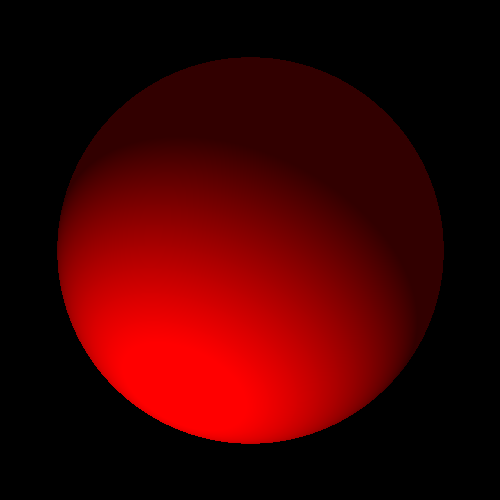
\includegraphics[scale=0.3]{boule.png}
	\caption{\label{fig:sphère} Application d’une lumière diffuse à une sphère rouge \protect \footnotemark }
\end{figure}
\footnotetext{http://linut.free.fr/omgspl0kuberwebloglolz0r/?2010/02/01/93-raytracer-que-la-lumiere-soit}

\paragraph{}
	Pour la création d’un anaglyphe, deux images espacées par une petite distance (qui correspond à la distance entre les deux yeux par exemple) sont générées. La composante rouge de l’une de ces images et la composante bleue de l’autre sont gardées et ensuite superposées dans une même image. Cette image est ensuite transformée en une image Rouge-Cyan, qui peut être visualisée à l’aide de lunettes Rouge-Bleue : l’image apparaît en trois dimensions.

\paragraph{}
	Pour la création d’un autostéréogramme, une image permettant d'observer un objet en relief par vision parallèle est générée. Cette image est obtenue à partir d'une texture de base ou de points aléatoires pour l'image de fond.

\paragraph{}
	Pour la création d’un flipbook, plusieurs images sont prises à intervalles réguliers par une caméra suivant un trajet prédéterminé dans ou autour de la scène. Le flipbook est visualisable en faisant rapidement défiler ces images tout en respectant l’ordre des prises de vue. Ce flipbook peut être transformé en GIF pour obtenir une visualisation animée des images.
